\documentclass{article}

\usepackage{geometry}
\usepackage{amsmath}
\usepackage{graphicx}
\usepackage{float}
\usepackage{amsthm}
\usepackage[dvipsnames]{xcolor}

%Short form to use stack_relative
\newcommand{\stck}{\stackrel{\longrightarrow}}

%A different version of the above 
\newcommand{\stckdet}[1]{\stackrel{{#1}}}

%We write a lot of relations between two events using the orderings, so a short form to use that
\newcommand{\reln}[3]{#1\stck{_{#2}}#3}

%We use a more detailed version of the above relation to indicate direct / indirect relations 

\newcommand{\reldet}[4]{#1\stckdet{_{#2}}{{\stck{_{#3}}}}#4}

%We also will introduce a short form to write an event belongs to some set
\newcommand{\event}[2]{#1\!\in\!#2}

%To make events and their type more close to each other
\newcommand{\typ}[1]{\textit{#1}}
\newcommand{\et}[2]{#1\!:\!\typ{#2}}

%Short form to write color text
\newcommand{\critic}[2]{\textcolor{#1}{\footnotesize #2}}

%Some preliminary latex commands to format writing theorems 

\newtheorem{lemma}{Lemma}

\newtheorem{theorem}{Theorem}[lemma]

\newtheorem{corollary}{Corollary}[theorem]

\newtheorem{definition}{Definition}

\newtheorem{property}{Property}


\begin{document}

    
        %\section{Objective}

        This whole document's purpose is to gain clarity over certain ideas that have been formulated in my head. 
        Usage of figures in this document will be heavy just to point out an intuition. 
        This document is also the first one written in latex in this respect. 
        The author of this article has taken a lot of effort just to start formulating ideas in latex format. 
        So if there are certain typos or errors in text, please do not mind and kindly report it to the author. 

    \section{Topic : Symmetry Reduction}

        Model checking is heavily relied upon as a testing tool for programs. 
        Given that programs are large model checking suffers from its constant problem of scalability. 
        Add to the above the introduction of concurrent programs, scalability becomes more of an issue. 
        
        However, to optimize model checking of concurrency, certain algorithms rely on reusing information from one execution. 
        In that sense, a certain dynamic programming approach is employed. 
        This dynamic approach is done to avoid certain redundant explorations, as well as to quickly discard further exploration of programs that violate the concurrent semantics.
        In the ones that I have read, which is called in literature as stateless model checking, storing the information of the writes each read operation has visited in some execution explored before is used to ensure optimal model checking. 
        
        But here the meaning of redundant is that of executions that the model checker has already explored. 
        There exists another kind of redundancy which is the fact that two different executions result in the same outcome. 
        This kind of redundancy relies more upon the semantic equivalence of two executions, rather than just syntactic. 

        One such instance of such redundancy is the equivalence(not equality) of exeuction graphs.
        The equivalence is sort of homomorphic as well as isomorphic. 
        Such kind of redundancy appears in concurrent programs due to different components of the program tasked to do mostly the same thing. (take for example, a client-server system)
        Such equivalent executions can be said to be symmetric to each other. 
        This means that one needs to explore just one of these executions to ensure the other symmetric ones are also explored.


        %\subsection{Graph and its Equivalence}

    \paragraph{Execution Graph}
    
        \begin{itemize}
            \item Has all the ordering relations defined by the axiomatic model (eg: happens-before, program-order)
            \item Each execution graph is unique
        \end{itemize}
    
    
    \paragraph{Equivalence}
        \begin{center}
            \emph{\textit{
                Two execution graphs E1 and E2 are symmetric / equivalent to each other, if we can swap thread identities of one of them to form the other. 
            }}  
        \end{center}

        In terms of ordering relations, swapping thread identities means: 
        \begin{itemize}
            \item Any reads-from relation established among events of the threads being swapped are also swapped.
            \item Reads-from relation from read of a thread being swapped to an outside write is changed such that the read is that of a swapped thread having the same relation with the write.   
        \end{itemize}

        \critic{blue}{There might be other derived relations, eg: happens-before, from-reads, etc. For now we only keep it restricted to reads-from relations.}

        In short, if we tag all the thread events by some number, simply changing the numbers by their swapped thread identities will ensure the above two. 

        \critic{blue}{Note that it could be the case that an execution has two threads to be of same code, but it may not reflect what it is in the original program. The equivalence is on the assumption that both threads do have equal code in both those  executions.}

    \paragraph{Example of swapping thread identities?}
        
        %Show an example here
        \begin{figure}[H]
            \centering
            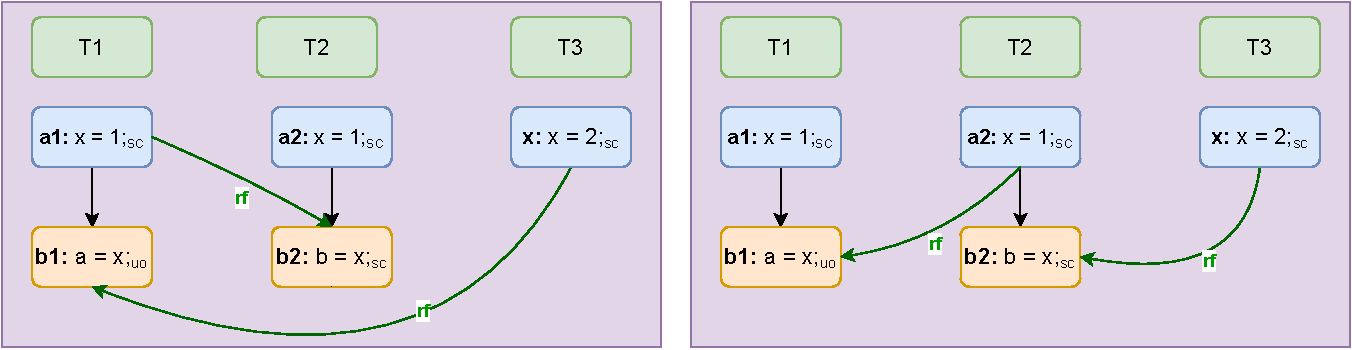
\includegraphics[scale=0.7]{Equivalence_Example.pdf}
            \caption{Example of two equivalent execution graphs}
        \end{figure}

        The two executions which are symmetric have the following reads-write relations. 
        \begin{align*}
            b1:x \ \wedge \ b2:a1 \\
            b1:a2 \ \wedge \ b2:x 
        \end{align*}

        Notice from the above figure that swapping thread identities of T1 and T2 implies jsut swapping $\{b1, b2\}$ and $\{a1, a2\}$.
        
        \critic{blue}{It took quite some time to have a clear picture of what swapping thread identities implied for us when looking at symmetric executions.}




        
        %\subsection{The Intuition}
    
    \paragraph{Order Between Symmetric Threads}
        \begin{itemize}
            \item Symmetric executions can be obtained by swapping thread identities.
            \item Hence without loss of generality, we can assume a single total order of all threads which have equal code.
            \item In this sense, each set of equal threads will have a total order assigned to them. 
        \end{itemize}

    \paragraph{Order between Events - Writes and Reads}
        \begin{itemize}
            \item Whenever a read-write relation implies an order between two writes in a symmetric thread, swapping their thread identities will give us a symmetric execution with the order between writes reversed.
            \item Hence maintaining a symmetric order between writes of threads with equal code might be useful. 
            \item However, do we need a fixed order between all writes or just among writes which are equal in each thread? 
            \item Order between reads may not be necessary as they are not implied due to any other ordering-relation.  
        \end{itemize}

    \critic{red}{Whether order between reads is important is something I have a counter example to show that it isn't. But  I am not able to understand why it isn't important.}

    \paragraph{Miscellaneous Points}

        About ordering between writes through reads. 
        \begin{itemize}
            \item Each thread's read can read from it's own write program ordered before it.
            \item Each thread's read can read from an outer write which implies an ordering between the writes in it's own thread and the external one from which it reads from. 
        \end{itemize}

        \begin{figure}[H]
            \centering
            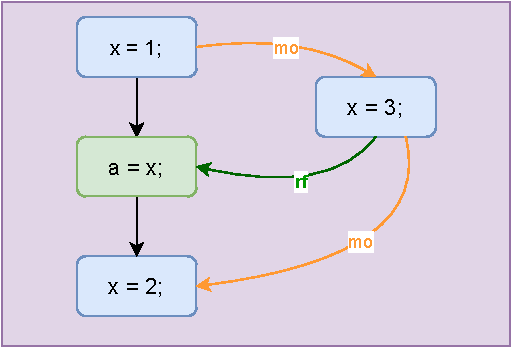
\includegraphics[scale=0.7]{WriteOrderImplied.pdf}
            \caption{Example showing that write orders(mo) implied due to the read-write(rf) relation.}
        \end{figure}




























   

        %\subsection{From Intuition to Examples}

    
    \emph{Any reads-from relation between a read (r) and a write (w) will be written as \textbf{r:w}} 


    \paragraph{Examples to show Write orders important}

        The following two examples show why having a symmetric order between same writes of each equal thread is important. 
        \begin{figure}[H]
            \centering 
            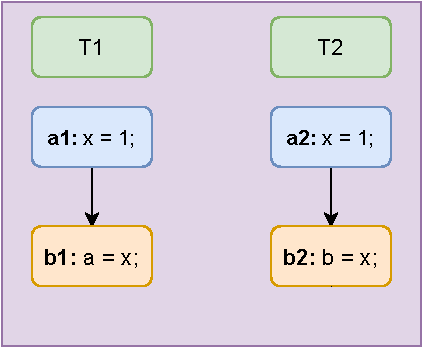
\includegraphics[scale=0.7]{Example1(2+wr).pdf}
            \caption{2+wr}
        \end{figure}

        The above example has the following possibilities of read-write relations that result due to an execution. Note that $b1:a2 , b2:a1$ is not possible due to coherence being our assumption. 
        \begin{align*}
            b1:a1 , b2:a1 \\ 
            b1:a1 , b2:a2 \\
            b1:a2 , b2:a2
        \end{align*}

        Observations:
        \begin{itemize}
            \item $b1:a1, b2:a1$ implies an ordering on the writes such that $a2$ occurs before $a1$.
            \item $b1:a2, b2:a2$ implies an ordering on the writes such that $a1$ occurs before $a2$.
            \item The above two executions are symmetric to each other as we can swap threads of one to get the other. 
            \item We need to fix an ordering between the equal writes of symmetric threads. 
        \end{itemize}
    
        \begin{figure}[H]
            \centering 
            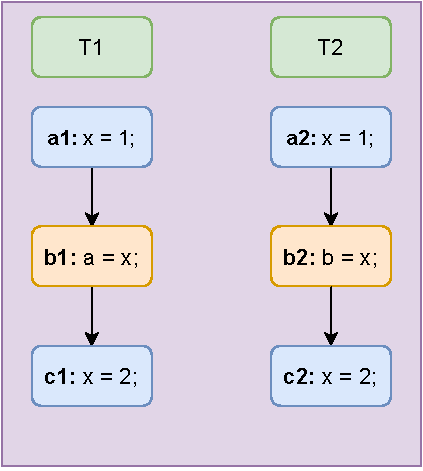
\includegraphics[scale=0.7]{Example2(2+wrw).pdf}
            \caption{2+wrw}
        \end{figure}
        
        The above example is an extension of the previous, by adding two writes following the reads to the same memory. Note that the outcome $b1:c2, b2:c1$ is not considered due to lack of Load-Buffering (I still think its Coherence). The following are the possible executions in terms of read-write relations. 

        \begin{align*} 
            b1:a1 , b2:a2 \\
            b1:a1 , b2:c1 \\ 
            b1:a2 , b2:a2 \\
            b1:a2 , b2:c1 \\
        \end{align*}

        Observations:
        \begin{itemize}
            \item $b1:c2, b2:a2$ is not counted as it implies that $c2$ is before $c1$, whose reverse is already covered by $b1:a1 , b2:c1$
            \item Same argument for why the case $b1:c2, b2:a1$ is not considered.
            \item A slight hint is given that ordering between reads also matters. (the case $b1:c2, b2:a2$ also implies $b2$ occurs before $b1$.) 
        \end{itemize}

    \paragraph{Examples to show Read Orders are(or may be) not important}

        \begin{figure}[H]
            \centering 
            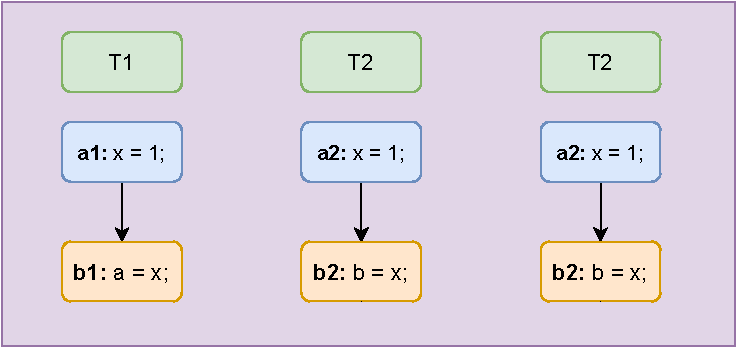
\includegraphics[scale=0.7]{Example3(3+wr).pdf}
            \caption{3+wr}
        \end{figure}


        The above example is extending the first example with another symmetric thread. It has the following executions covered using our insight from the previous examples. 
        \begin{align*}
            b1:a1 , b2:a2 , b3:a3 \\
            b1:a1 , b2:a3 , b3:a3 \\
            b1:a2 , b2:a2 , b3:a3 \\
            b1:a2 , b2:a3 , b3:a3 \\
            b1:a3 , b2:a2 , b3:a3 \\
            b1:a3 , b2:a3 , b3:a3
        \end{align*}

        Observation:
        \begin{itemize}
            \item $b1:a1 , b2:a3 , b3:a3$ and $b1:a2 , b2:a2 , b3:a3$ appear to be symmetric, but considering the total order between equal writes also as part of execution, they are not symmetric, rather they are unique. 
            \item  $b1:a3 , b2:a2 , b3:a3$ is a case we would not have covered, if we enforced an order between reads, as it would then mean that $b2$ can only read from $a3$. 
            \item Enforcing read orders prevent the above case. The above case is valid because $b2:a2$ implies no ordering between writes, hence the order between $a1$ and $a2$ can be left to us. 
            \item \textcolor{red}{However, the above case is symmetric to $b1:a2 , b2:a2 , b3:a3$; swap identities of thread $T2$ and $T3$}
            \item This strengthens our intuition of equivalent executions that can be obtained by swapping thread identities, due to reversing implied orders between writes. 
        \end{itemize}

        \critic{red}{Not enforcing an order between reads, may have issues about completeness, meaning we might cover a few redundant explorations.}

        \begin{figure}[H]
            \centering
            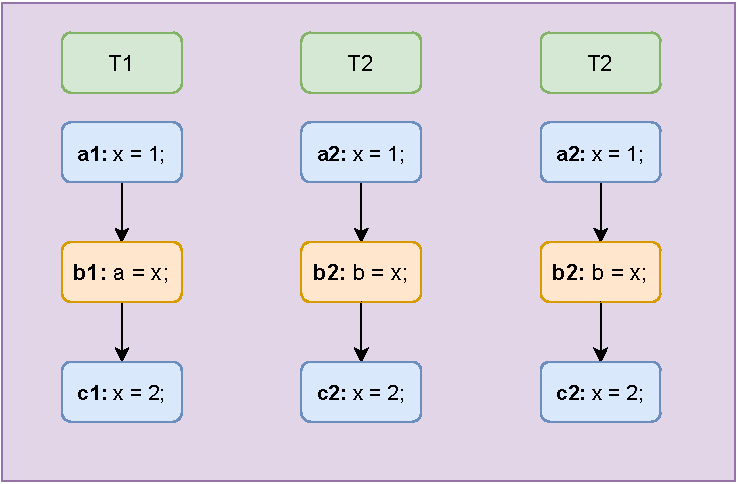
\includegraphics[scale=0.7]{Example4(3+wrw).pdf}
            \caption{3+wrw}
        \end{figure}

        The above example is extending the previous with additional writes to each thread. The possible executions are many, hence not all of them will be elicited, but ones of focus: 
        
        \begin{align*}
            b1:a1 , b2:a3 , b3:c1 \\
            b1:a3 , b2:a2 , b3:c2 \\
            b1:a1 , b2:a2 , b3:c1 \\
            b1:a2 , b2:a2 , b3:c1 \\
        \end{align*}

        Observation:
        \begin{itemize}
            \item $b1:a1 , b2:a3 , b3:c1$ would not be explored if we consider $b1:a1 , b2:a3 , b3:a3$ to be symmetric to $b1:a2 , b2:a2 , b3:a3$. Considering them symmetric would make us assume that when $b1:a1$, then $b2$ cannot read from any outside write other than that of $T1$. 
            \item $b1:a3 , b2:a2 , b3:c2$ would not be explored if we ordered the reads too. However, it is also the case that $b1:a1 , b2:a3 , b3:c1$ is symmetric to this (just swap thread identities of $T1$ and $T2$). Further investigation is needed. This tells our approach may not be complete. 
            \item \textcolor{red}{$b1:a1 , b2:a2 , b3:c1$ is symmetric to $b1:a1 , b2:a2 , b3:c2$ , but it does not violate our requirement of implied write orders.}
            \item \textcolor{red}{$b1:a2 , b2:a2 , b3:c1$ is symmetric to $b1:a3, b3:a3, b2:c1$, but it does not violate our requirement of implied write orders.} 
            \item Conclusion from this example is that implied write orders is not complete. 
        \end{itemize}

        
    \paragraph{Examples to show affects of external non-symmetric writes}
        %Now consider extending the first example with another non symmetric thread 2+wr+w
        \begin{figure}[H]
            \centering 
            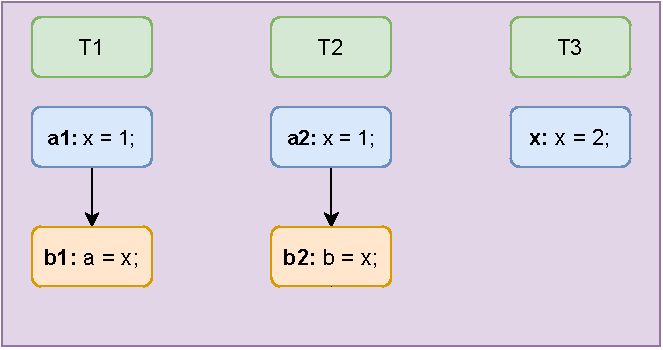
\includegraphics[scale=0.7]{Example5(2+wr+w).pdf}
            \caption{2+wr+w}
        \end{figure}

        The above example is the first program extended with another non-symmetric thread having a write to same memory. We elicit the following possible executions, catering to our rules for implied write orders: 
        \begin{align*}
            b1:a1 , b2:a2 \\
            b1:a1 , b2:x \\
            b1:a2 , b2:a2 \\
            b1:a2 , b2:x \\
            b1:x , b2:x \\
            b1:x , b2:a2
        \end{align*}

        Observations: 
        \begin{itemize}
            \item There is no restriction on order with the write $x$ and $a1, a2$.
            \item $b1:x , b2:a2$ is symmetric to $b1:a1 , b2:x$. But both of these explored do not violate implied write orders. 
            \item $b1:x , b2:a2$ can correspond to an order of writes being $a1->x->a2$ still respecting the order of writes that must hold. Whereas, $b1:a1 , b2:x$ can correspond to the order of writes being $a1->a2->x$ also respecting the order of writes that must hold. 
        \end{itemize}

        \begin{figure}
            \centering
            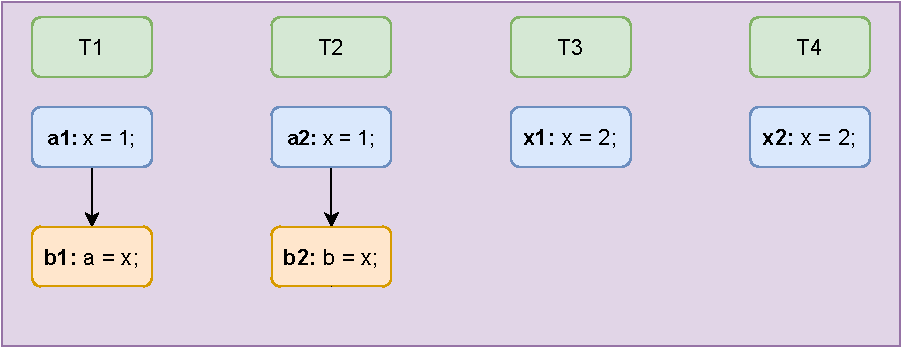
\includegraphics[scale=0.7]{Example6(2+wr+2+w).pdf}
        \end{figure}

       
        The above example is with two symmetric sets of threads. We have the following executions possible keeping our implied writes rule intact. 

        \begin{align*}
            b1:a1 , b2:a2 \\
            b1:a1 , b2:x1 \\
            b1:a1 , b2:x2 \\
            b1:a2 , b2:a2 \\
            b1:a2 , b2:x1 \\
            b1:a2 , b2:x2 \\
            b1:x1 , b2:a2 \\
            b1:x1 , b2:x2 \\ 
            b1:x2 , b2:a2 \\
            b1:x2 , b2:x2 \\
            b1:x2 , b2:x1
        \end{align*}

        Observation:
        \begin{itemize}
            \item \textcolor{red}{$b1:x1 , b2:x2$ is symmetric to $b1:x2 , b2:x1$, yet these two do not violate the implied writes.} rules. 
        \end{itemize}
        
        Notice that we do not have the case $b1:x2 , b2:x1$, as it implicitly violates the ordering constraint that $b1$ occurs before $b2$.

        (Still ongoing, examples with operations to multiple memory segments need to be analyzed)

        %Lastly consider the case 3+wrw+w

        %Keep this section open to more interesting examples

        \subsection{From Examples to Precise Rules}

    \paragraph{Notations}
        \begin{itemize}
            \item $T_i$ denotes thread number $i$.
            \item $T_i \equiv T_j$ means both threads have same code.
            \item $w_i^j$ is the $j^{th}$ event in thread $i$ which is a write.
            \item $r_i^j$ is the $j^{th}$ event in thread $i$ which is a read. 
        \end{itemize}

    
    \paragraph{A few definitions for our use}

    \begin{definition}{Program Order(\emph{po})}
        Total order between events in the same thread. Respects the execution order between events in the same thread. 
    \end{definition}

    \begin{definition}{Symmetric Memory Order (\emph{smo})}
        A strict partal order between writes in a set of symmetric threads. Consider a set of symmetric threads $T_1 \equiv T_2 \equiv ... \equiv T_n$. Each of these threads have exactly one read event, and multiple write events, all to the same memory, say $x$. 

        Then each write in the above threads are involved in a symmetric order, such that. 
        \begin{align*}
            \forall i \in [0, n-1] \ . \ \reln{w_i^j}{smo}{w_{i+1}^j}
        \end{align*}
        Where j denotes the $j^{th}$ event in any of the threads, which is a write.
    \end{definition}

    \critic{blue}{Perhaps should put examples for the above defintion.}

    \begin{definition}{Reads-From (\emph{rf})}
        Binary relation that links a read to a write from which its value comes. Note that for our purpose, this relation is functional.
        For example, if a read $r_i^j$ gets its read value from write $w_k^l$, then we have the relation. 
        \begin{align*}
            \reln{w_k^l}{rf}{r_i^j}
        \end{align*}
    \end{definition}

    \paragraph{Main Rule}
        Using the above setup, our intention is to explore lesser execution graphs leveraging the symmetry that can result due to swapping of thread identities. For this, we enforce a restriction on possible $\stck{_{rf}}$ relations that are to be considered \emph{valid}. A valid $\stck{_{rf}}$ relation is one that respects the following \textbf{irreflexivity constraints}. 
        \begin{align*}
            smo;rf;po \\
            smo;po;rf^{-1} 
        \end{align*}

        \critic{blue}{We can add here more as we go about to prove completeness.}

        \critic{red}{Recall examples to show how our analysis through examples satisfy the above irreflexivity constraint.}

        



        \subsection{Soundness of the rules above}

    To prove soundness, we first define the following: 

    \begin{definition}{Implied Write Order(\emph{iwo})}
        Binary relation between any two \emph{distinct} writes, derived through the following two sequential conposition:  
        \begin{align*}
            w_i^j;po;rf^{-1};w_k^j \\
            w_i^j;rf;po;w_k^j 
        \end{align*}
    \end{definition}

%---------------------------------------------------------------------------------------------------------------------------------    

    \begin{property}{Simplified irreflexivity rule}
        
        The irreflexivity constraint rule is equivalent to the following irreflexivity condition 
        \begin{align}
            smo;iwo
        \end{align}
    \end{property}

    \begin{proof}
        Expanding for implied write order as per the definition, gives us the following two sequential compositions. 
        \begin{align}
            smo;w_i^j;po;rf^{-1};w_k^j \\
            smo;w_i^j;rf;po;w_k^j 
        \end{align}
        From the definiton of symmetric order, the above can be simplified to
        \begin{align}
            smo;po;rf^{-1} \\
            smo;rf;po 
        \end{align}
        Hence, proving our property. 
    \end{proof}

%-----------------------------------------------------------------------------------------------------------------------------------

    \begin{property}
        No write order is implied when a read reads from its own thread's write
    \end{property}

    \begin{proof}
        If the read is from its own thread's write, then we can infer that $i=k$ in both the sequential compositions. Hence  
        \begin{align*}
            w_i^j;rf;po;w_i^j \\
            w_i^j;po;rf^{-1};w_i^j
        \end{align*} 
        which gives us $\reln{w_i^j}{iwo}{w_i^j}$.
        Since implied write orders are only between distinct writes, the property is proven.  
    \end{proof}
        
%-------------------------------------------------------------------------------------------------------------------------------------

    \begin{property}
        Implied write orders between two symmetric threads are reversed when they are swapped.
    \end{property}
        
    \begin{proof}
        Considering first sequential composition, i.e. $w_i^j;rf;po;w_k^j$, expanding gives us the following binary relations involved:
        \begin{align}
            \reln{w_i^j}{rf}{r_k} \\
            \reln{r_k}{po}{w_k^j}
        \end{align}
        Swapping thread identities involves swapping the indices $i$ and $k$ for each event, thus giving us 
        \begin{align}
            \reln{w_k^j}{rf}{r_i} \\
            \reln{r_i}{po}{w_i^j}
        \end{align}
        Through sequential composition of the above, we get $w_k^j;rf;po;w_i^j$, which by definition is $\reln{w_k^j}{iwo}{w_i^j}$.

        The argument is symmetric for the second sequential composition. 
    \end{proof}
        
%-------------------------------------------------------------------------------------------------------------------------------------

    \begin{property}
        There are at most two implied write orders between writes of two threads.
    \end{property}
        
    \begin{proof}
        Consider two threads $T_i$ and $T_k$. Suppose we have one implied write order between one of their writes, i.e. 
        \begin{align}
            \reln{w_i^j}{iwo}{w_k^j}.    
        \end{align}
        Expanding as per the first sequential composition gives us 
        \begin{align}
            w_i^j;po;rf^{-1};w_k^j
        \end{align}
        which also indicates a $\stck{_{rf}}$ with $T_i$'s read and that the writes involved in the composition are above the respective reads.

        Now suppose we have an implied write order between another set of writes, i.e.
        \begin{align}
            \reln{w_i^l}{iwo}{w_k^l}.    
        \end{align}
        Expanding as per the first sequential composition of implied write order is not possible as $\stck{_{rf}}$ is functional. Hence, using the second we have
        \begin{align}
            w_i^j;rf;po;w_k^j 
        \end{align}  
        which also indicates a $\stck{_{rf}}$ with $T_i$'s read that the writes involved in the composition are below the respective reads.

        Since both reads are now involved in a $\stck{_{rf}}$ relation, and since this relation is functional, we cannot have any more implied write orders between $T_i$ and $T_j$, thus verifying our property. 

        \critic{blue}{Better written in contrast to previous argument.}
        \critic{red}{However, is it necessary to show by contradiction?}
    \end{proof}
        
%--------------------------------------------------------------------------------------------------------------------------------------

    \begin{property}
        Implied write ordes between two threads are either all compliant with $stck{_{smo}}$ or they are all not
    \end{property}

    \begin{proof}
        
        If each read reads from its own write, we have no implied write order established, thus maintaining the property. 

        For cases where implied write orders are established, without loss of generality, let us consider one between writes above the read are compliant with $stck{_{smo}}$:
        \begin{align}
            \reln{w_i^j}{iwo}{w_k^j} \ \wedge \ \reln{w_i^j}{smo}{w_k^j}
        \end{align}
        The other set of implied write order, if established can only be between writes below the read. Suppose we have such an order but not compliant with $stck{_{smo}}$:
        \begin{align}
            \reln{w_k^l}{iwo}{w_i^l} \ \wedge \ \reln{w_i^l}{smo}{w_k^l}
        \end{align}
        Upon expanding using the second sequential composition (because writes are below the read), we get
        \begin{align}
            w_k^l;rf;po;w_i^l 
        \end{align}
        But this implies another $\stck{_{rf}}$ relation with $T_i$'s read, which violates the functional property of it. Hence we can only have an implied write order compliant with $stck{_{smo}}$.
        \begin{align}
            \reln{w_i^l}{iwo}{w_k^l} \ \wedge \ \reln{w_i^l}{smo}{w_k^l}
        \end{align}

        \critic{red}{Not sure if we need to show that the compliant relation also holds as it only brings an rf realtion with $T_k$'s read, which wanst established before.}

        The opposite case would make both the implied write orders requiring to not be compliant, thus by symmetry completing our proof. 
    \end{proof}

%-------------------------------------------------------------------------------------------------------------------------------------- 
        
    \begin{property}
        Implied write orders are acyclic
    \end{property}

    \begin{proof}
        %By Contradiction 
        Suppose a cycle exists. Then without loss of generality, we can consider the cycle composed of 3 writes.
        \begin{align}
            \reln{w_i^j}{iwo}{w_k^j} \ \wedge \reln{w_k^j}{iwo}{w_l^j} \ \wedge \reln{w_l^j}{iwo}{w_i^j}  
        \end{align}
        
        If these writes are above the read, then we have the following relations that result in the above cycle.
        \begin{align}
            \reln{w_i^j}{po}{r_i} \ \wedge \ \reln{r_i}{rf^{-1}}{w_k^j} \\
            \reln{w_k^j}{po}{r_k} \ \wedge \ \reln{r_k}{rf^{-1}}{w_l^j} \\
            \reln{w_l^j}{po}{r_l} \ \wedge \ \reln{r_l}{rf^{-1}}{w_i^j} 
        \end{align}
        The above relations form a cycle thus violating $po \cup rf^{-1} \ \text{acyclic}$ rule for coherence and hence violating coherence.
        
        If these writes are below the read, then we have the following relations that result in the above cycle.
        \begin{align}
            \reln{w_i^j}{po}{r_i} \ \wedge \ \reln{r_i}{rf}{w_k^j} \\
            \reln{w_k^j}{po}{r_k} \ \wedge \ \reln{r_k}{rf}{w_l^j} \\
            \reln{w_l^j}{po}{r_l} \ \wedge \ \reln{r_l}{rf}{w_i^j} 
        \end{align}
        The above relations form a cycle thus violating $po \cup rf \ \text{acyclic}$ rule for coherence and hence violating coherence.

        Because both cases violate coherence, we conclude that $\stck{_{iwo}}$ must be acylic. 

        \critic{blue}{A bit better written compared to the previous proofs}
    \end{proof}

%---------------------------------------------------------------------------------------------------------------------------------------

    \critic{red}{Need to also prove the properties of incmoing or outgoing write orders.}

    \subsubsection{Soundness}

        To prove that our rules our sound, we show that for every implied write order such that $smo;iwo$ is reflexive, we can swap the corresponding thread identities to reverse the write order between them, thus respectiing our irreflexivity constraint. However, we must ensure that once write orders are "fixed" in this fashion, they remain fixed, i.e. the relation cannot appear again to be wrong. Once we show this, we also need to show that this holds in general given multiple sets of equal writes. 
        
        \paragraph{Part1}
            For a given set of equal writes, once an implied write order is fixed, it remains fixed. 
            (A more formal statement required)
        \begin{proof}
            %Proof by contradiction 
            Suppose we have one implied write order which is correct / fixed between writes $w_i^j$ and $w_k^j$.
            \begin{align}
                \reln{w_i^j}{iwo}{w_k^j}
            \end{align}
            Without loss of generality, suppose these writes are above the read. We then divide our concern into two parts, one with implied write orders with $w_i^j$ which are wrong and the second with those of $w_k^j$.

            Case1: 
            Because $w_i^j$ is a write above read and $\reln{w_i^j}{iwo}{w_k^j}$, other implied write orders with $w_i^j$ can be of the form:
            \begin{align}
                \reln{w_m^j}{iwo}{w_i^j}
            \end{align}
            If this implied order is wrong, swapping thread identities will  give us the following relations 
            \begin{align}
                \reln{w_i^j}{iwo}{w_m^j} \ \wedge \ \reln{w_m^j}{iwo}{w_k^j}  
            \end{align}  
            Here, there is no implied write order relation between $w_i^j$ and $w_k^j$, hence we can consider them as remaining fixed. 
            If the implied order between $w_m^j$ and $w_k^j$ is wrong, swapping it will result in the following relations
            \begin{align}
                \reln{w_i^j}{iwo}{w_k^j} \ \wedge \ \reln{w_k^j}{iwo}{w_m^j}  
            \end{align}  
            Here, the implied write order between $w_i^j$ and $w_k^j$ remains the same. Thus, for this case, we can conclude that the relation remains "fixed".

            Case2: 
            Other implied write orders with $w_k^j$ can be of the forms:
            \begin{align}
                \reln{w_m^j}{iwo}{w_k^j} \\ 
                \reln{w_k^j}{iwo}{w_m^j}
            \end{align} 
            The first form is symmetric to our Case1, hence we only consider the second form. 

            If this implied write order is wrong, swapping thread identities will give us the following relations. 
            \begin{align}
                \reln{w_i^j}{iwo}{w_m^j} \ \wedge \ \reln{w_k^j}{iwo}{w_m^j}
            \end{align}
            Here, there is no implied write order relation between $w_i^j$ and $w_k^j$, hence we can consider them as remaining fixed. 

            But if the implied write order between $w_m^j$ and $w_i^j$ is wrong, swapping them will give us 
            \begin{align}
                \reln{w_m^j}{iwo}{w_i^j} \ \wedge \ \reln{w_k^j}{iwo}{w_i^j}  
            \end{align}
            thus making our claim invalid. To show that this state is not possible, note firstly that from the initial configuration, we can infer if $\reln{w_m^j}{iwo}{w_k^j}$ is wrong:
            \begin{align}
                \reln{w_i^j}{smo}{w_k^j} \ \wedge \ \reln{w_k^j}{smo}{w_m^j}
            \end{align} 
            Because $smo$ is a total order w.r.t. one set of writes, we have by transitivity. 
            \begin{align}
                \reln{w_i^j}{smo}{w_m^j}
            \end{align}
            After swapping threads $T_k$ and $T_m$, we get $\reln{w_i^j}{iwo}{w_m^j}$ which respects the irreflexivity constraint $smo;iwo \ \text{scyclic}$. Hence, this implied write order is not wrong. Thus we cannot have the case which results in $\reln{w_k^j}{iwo}{w_i^j}$.  

            Thus, for a given set of equal writes, once an implied write order is fixed, it remains fixed.
        \end{proof}

        \paragraph{Part2}
        For a given set of writes, any new implied write order introduced is new and, if wrong, it can be fixed and will remain fixed. 
        (A more formal statement required)
        \begin{proof}
            Suppose, for a given set of equal writes, say of the form $w^j$ all the implied write orders are fixed. Without loss of generality, let us consider them to be wrties above the read. We consider two threads $T_i$ and $T_k$, between which an implied write order is wrong. Let those writes be $w_i^l$ and $w_k^l$. 

            Once again, without loss of generality, let us consider the symmetric memory order between writes of $T_i$ and $T_k$ to be of the form $\reln{w_i}{smo}{w_k}$. Thus we have 
            \begin{align}
                \reln{w_i^j}{smo}{w_k^j} \ \wedge \ \reln{w_i^l}{smo}{w_k^l}
            \end{align}

            Because we assume write order is wrong between $w_i^l$ and $w_k^l$, by property x (forgot the number), and by our assumptions that implied write orders among $w^j$ are fixed, we have 
            \begin{align}
                \reln{w_k^l}{iwo}{w_i^l}
            \end{align} 
            There cannot be an implied write order between $w_i^j$ and $w_k^j$, as if there were, then it would be the fixed one, and by property y (forgot number), that between $w_i^l$ and $w_k^l$ would also be the fixed one. 

            \textbf{Case1: $w^l$ is below the read.}
            
                Part1: There exists an implied write order between another write $w^j$ and $w_i^j$. 

                    Because $w^l$ is below the read and $\reln{w_k^l}{iwo}{w_i^l}$, $w_i^j$ can only be involved in implied write orders of the form 
                    \begin{align}
                        \reln{w^j}{iwo}{w_i^j}
                    \end{align}
                    From this and the fact that impleid write orders of $w^j$ are fixed already, we have
                    \begin{align}
                        \reln{w^j}{smo}{w_i^j} 
                    \end{align} 
                    By transitivity, we then have $\reln{w^j}{smo}{w_k^j}$.

                    If we swap $T_i$ and $T_k$ to fix $\reln{w_k^l}{iwo}{w_i^j}$, we have the following new relations.
                    \begin{align}
                        \reln{w_i^l}{iwo}{w_k^j} \\
                        \reln{w^j}{iwo}{w_k^j}
                    \end{align}
                    Both these relations repsect our irreflexivity constraint. Hence, maintaining that new implied write order relations with $w^j$ are not wrong.
                    
                Part2: There exists an implied write order between another write $w^j$ and $w_k^j$. 
                    
                    $w_k^j$ can be involved in implied write orders of the form
                    \begin{align}
                        \reln{w_k^j}{iwo}{w^j} \\
                        \reln{w^j}{iwo}{w_k^j} 
                    \end{align}
                    The first is symmetric to Part1, hence we only consider the second form. 

                    On swapping $T_i$ and $T_k$, we get the following new relations:
                    \begin{align}
                        \reln{w_i^l}{iwo}{w_k^j} \\
                        \reln{w^j}{iwo}{w_i^j}
                    \end{align}

                    The second form may not be compliant to the irreflexivity condition, hence can be a new implied relation which is wrong. To show that this is new and could have not occurred before while swapping threads to fix implied write orders of $w^j$, consider the original configuration we have 
                    \begin{align}
                        \reln{w_i^j}{smo}{w_k^j} \ \wedge \ \reln{w^j}{iwo}{w_k^j}
                    \end{align}
                    For $\reln{w^j}{iwo}{w_k^j}$ to have been there before, there must be a write $x$, say, such that 
                    \begin{align}
                        \reln{x}{iwo}{w_i^j} \ \wedge \ \reln{x}{iwo}{w^j}
                    \end{align}
                    So that while swapping to reverse relation between $x$ and $w^j$ or $x$ and $w_i^j$, we can get our new relation. But such an $x$ cannot exist, as by property z (forgot number), writes above read, can only have one relation of the form $\reln{x}{iwo}{y}$ where $y$ is another equal write. Hence, such a relation could have not been there before, and hence was not fixed. 

                    Now that this new relation exists, fixing it, will keep it remain fixed, by our first part of proof (label them please). 
                    
            
            \textbf{Case2: $w^l$ is above the read.}
                
                Part1: There exists an implied write order between another write $w^j$ and $w_i^j$.

                Since $T_i$'s read is still free, $w_i^j$ can have implied write orders with $w^j$ of the form
                \begin{align}
                    \reln{w_i^j}{iwo}{w^j} \\
                    \reln{w_i^j}{iwo}{w^j} 
                \end{align}

                \critic{blue}{This case is symmetric to the above, so we will write it later.}

                For the second form, while we swap threads $t_i$ and $T_k$, we get the following new relations (correct his)
                \begin{align}
                    \reln{w_i^l}{iwo}{w_k^j} \\
                    \reln{w_k^j}{iwo}{w^j}
                \end{align}
                The second relation may not be compliant to the irreflexivity condition, hence can be a new implied relation which is wrong. To show that this is new and could have not occurred before while swapping threads to fix implied write orders of $w^j$, consider the original configuration we have 
                \begin{align}
                    \reln{w_i^j}{smo}{w_k^j} \ \wedge \ \reln{w_i^j}{iwo}{w^j}
                \end{align}

                For $\reln{w^j}{iwo}{w_k^j}$ to have been there before, we need an event $x$ to connect, hence by possible implied write orders one can have with $w^j$ and $w_k^j$, we need an $x$ such that one of the conditions below hold
                \begin{align}
                    \reln{w^j}{iwo}{x} \ \wedge \ \reln{x}{iwo}{w_k^j} \\ 
                    \reln{x}{iwo}{w^j} \ \wedge \ \reln{x}{iwo}{w_k^j}
                \end{align}

                The first condition violates coherence ($po \cup rf_{-1}$ acylcic), while the second condition cannot hold as such an event $x$ cannot exist due to property x (number the properties).
                
                Thus, such a relation could have not been there before, and hence was not fixed. 

                Now that this new relation exists, fixing it, will keep it remain fixed, by our first part of proof (label them please).

                \critic{red}{Write the above argument better please.}

        \end{proof}

        

   

\end{document}
    


